\documentclass[10pt,twocolumn]{article}

\usepackage[utf8]{inputenc}
\usepackage[T1]{fontenc}
\usepackage{lmodern}
\usepackage[margin=0.68in,columnsep=0.24in]{geometry}
\usepackage{amsmath,amssymb,amsfonts}
\usepackage{graphicx}
\usepackage{booktabs}
\usepackage{multirow}
\usepackage{array}
\usepackage{microtype}
\usepackage{xcolor}
\usepackage{titlesec}
\usepackage[font=small,labelfont=bf]{caption}
\usepackage{hyperref}

\hypersetup{
  colorlinks=true,
  linkcolor=blue!60!black,
  citecolor=green!45!black,
  urlcolor=blue!70!black,
  pdftitle={Compute-Optimal Neural MCTS on Edge NPUs},
  pdfauthor={Musheer Alam}
}

\titleformat{\section}{\normalfont\large\bfseries\raggedright}{\thesection}{0.6em}{}
\titleformat{\subsection}{\normalfont\normalsize\bfseries\raggedright}{\thesubsection}{0.6em}{}
\titlespacing*{\section}{0pt}{1.1em}{0.45em}
\titlespacing*{\subsection}{0pt}{0.85em}{0.3em}

\setlength{\parskip}{0.22em}
\setlength{\abovecaptionskip}{5pt}
\setlength{\belowcaptionskip}{4pt}
\emergencystretch=1.5em

\title{\textbf{Compute-Optimal Neural MCTS on Edge NPUs: Sensitivity-Guided Hybrid Quantization, Distributional Value Heads, and Co-Resident Graph Gear-Shifting}}

\author{
  Musheer Alam \\
  \small Independent Researcher \\
  \small \url{https://github.com/Musheer360/NeuraChess}
}

\date{}

\begin{document}

\twocolumn[
  \begin{@twocolumnfalse}
    \maketitle
    \vspace{-1.4em}
    \begin{abstract}
      \noindent Modern neural Monte Carlo Tree Search (MCTS) engines such as AlphaZero and Leela Chess Zero rely on 250--700\,W datacenter GPUs with high-bandwidth memory and dynamic batching. Migrating neural MCTS onto a 3\,W consumer edge neural processing unit (Intel AI Boost NPU~3720) exposes a fundamentally different hardware regime governed by ahead-of-time static tensor compilation, a tight ${\sim}4$\,MB on-chip CMX SRAM ceiling, and sequential tree-expansion dependencies that break standard quantization and scaling recipes. We present \textsc{NeuraChess} (\texttt{v1.1.0}), a hardware--algorithm co-designed chess engine pairing a C++23 AVX2/BMI2 Struct-of-Arrays PUCT engine with sensitivity-guided mixed-precision NPU inference. First, layerwise quantization profiling across a 10-block Squeeze-and-Excitation ResNet reveals a bimodal failure mechanism: quantizing the final residual block (\texttt{block\_9}) triggers a $>9\times$ policy KL divergence spike ($0.013042$), whereas \texttt{block\_1} causes a $0.926$ maximum value inversion. Keeping outer blocks (\texttt{0, 1, 8, 9}), Squeeze-and-Excitation gates, residual skip additions, and heads in FP16 while applying joint Middle-Block (\texttt{2..7}) W8A8 quantization-aware training (QAT) and zero-retraining weight souping reverses a $-12\%$ to $-20\%$ post-training quantization (PTQ) collapse into a $+19.6\%$ search throughput gain ($3{,}891$ vs.\ $3{,}254$\,NPS) and a statistically significant $+56.5$\,Elo head-to-head victory over Pure FP16 across 180 paired NPU games (pentanomial SPRT $\mathrm{LLR} = +3.8313 > +2.9444$, \texttt{ACCEPT\_H1}). Second, replacing scalar $\tanh$ MSE regression with a 64-bin Histogram Loss (\texttt{HL-Gauss-64}) plus Moves-Left Head (MLH) adds only $+0.012$\,ms ($+0.19\%$) on NPU~3720 while trained via a decoupled Spot FinOps pipeline for $\$63.59$ cumulative cloud spend. Third, co-resident static-graph gear-shifting ($B\in\{1,4,8,16\}$ in $59.09$\,MB NPU memory) accelerates Mate-in-3 search by $3.15\times$ and boosts 50\,ms/100\,ms puzzle accuracy by $+8.0\%$/$+7.0\%$, while ablations establish why static $B=16$ double-buffering wins under warm pondered trees; we further introduce a 4-gear clock-aware UCI allocator, MCTS early-stopping, and Syzygy DTZ zeroing conversion that eliminate time-pressure flagging in live $1+1$ bullet play. Finally, function-preserving depth expansion (\texttt{10x192}\,$\to$\,\texttt{12x192}, Step-0 drift $0.000$) maps the CMX SRAM Pareto cliff, accompanied by rigorous negative results on 37.85\,ns bitboard Static Exchange Evaluation (SEE) prior shaping and 50-node async dispersion. End-to-end, \textsc{NeuraChess} achieves $2{,}992$ mean implied \texttt{UCI\_Elo} across 150 Stockfish~19 ladder games, surges from $37.50\%$ to $83.75\%$ in fixed-node (\texttt{nodes 3500}) crossover play, and solves $95.65\%$ of $1{,}979$ clean Lichess puzzles at 800 nodes.
    \end{abstract}
    \vspace{1.2em}
  \end{@twocolumnfalse}
]

% =========================================================================
\section{Introduction}
% =========================================================================

The paradigm introduced by AlphaZero~\cite{silver2018alphazero} and scaled by community efforts such as Leela Chess Zero (\textsc{Lc0})~\cite{lc02024} demonstrated that coupling deep policy--value neural networks with Predictor Upper Confidence Trees (PUCT)~\cite{rosin2011puct} yields grandmaster- and superhuman-level strategic play. Yet the systems assumptions underlying server-GPU neural MCTS do not transfer to ultra-low-power consumer edge accelerators. On a datacenter GPU (e.g., NVIDIA L40S or H100), hundreds of watts of thermal headroom, gigabytes of HBM bandwidth, and large asynchronous search batches ($B=64$--$512$) amortize kernel launch latency and absorb transformer attention overheads. By contrast, a modern laptop-integrated neural processing unit---specifically the Intel AI Boost NPU~3720 inside Intel Core Ultra (Meteor Lake) processors operating at roughly 3\,W---enforces three structural constraints that directly reshape both neural architecture and tree search:

\begin{enumerate}
  \item \textbf{Static Ahead-of-Time Graph Compilation:} OpenVINO's NPU compiler lowers fixed-shape graphs into monolithic hardware command blobs~\cite{openvino2024}. Dynamic control flow, variable batch sizes, and runtime shape recompilation are prohibitively expensive during millisecond-scale chess moves, requiring either fixed batch shapes or explicit co-resident multi-shape compilation.
  \item \textbf{Tight On-Chip SRAM Capacity (${\sim}4$\,MB CMX):} When weights and intermediate feature maps exceed the NPU's on-chip Connection Matrix (CMX) scratchpad, the compiler inserts DMA spills to shared system LPDDR memory. As we show empirically in Section~\ref{sec:scaling}, this induces a sharp latency cliff beyond ${\sim}7.5$--$8.0$\,M parameters, invalidating monotonic GPU scaling intuition where deeper models consistently win under fixed wall-clock budgets.
  \item \textbf{Iterative Sequential Tree Dependencies:} Unlike throughput-bound vision classification or autoregressive LLM prefill, PUCT search is an iterative feedback loop in which batch $t+1$'s leaf selection depends on value backups from batch $t$. Increasing batch size from $B=16$ to $B=32$ or $B=64$ boosts raw positions per second on the NPU but degrades actual playing strength to $26.56\%$ ($8.5/32$) and $0.00\%$ ($0/16$) against $B=16$ due to virtual-loss collision staleness and reduced sequential ply depth. Similarly, scaled dot-product attention transformers incur severe hardware stalls on NPU~3720 ($723$--$1{,}351$\,pos/s), running $2.8\times$--$5.3\times$ slower than convolutional Squeeze-and-Excitation (SE) ResNets ($3{,}831$\,pos/s at \texttt{10x128})~\cite{he2016resnet,hu2018senet}.
\end{enumerate}

Compounding these hardware constraints, neural MCTS exhibits extreme sensitivity to uniform post-training quantization (PTQ)~\cite{nagel2021whitepaper}. While 1--2\% top-1 degradation is often tolerable in image classification, a single $0.97$ value-head sign inversion on a tactical leaf propagates directly through PUCT backup and causes immediate game-losing blunders. Moreover, because board-plane neural networks lack any representation of wall-clock pressure, deploying a neural engine into real-time blitz and bullet controls exposes subtle systemic interactions between the UCI clock allocator, MCTS termination criteria, pondering pipelines, and endgame tablebase move ordering.

This paper systematically resolves these challenges in \textsc{NeuraChess} (\texttt{v1.1.0}) and makes five primary contributions:
\begin{itemize}
  \item \textbf{Heterogeneous P-Core + NPU Co-Design \& Clock-Aware Real-Time Control (Section~\ref{sec:system}):} We quantify the $91.44\%$ CPU-idle asymmetry on Core Ultra + NPU~3720, detail a C++23 AVX2/BMI2 Struct-of-Arrays (SoA) PUCT engine with 5-piece Syzygy WDL/DTZ integration ($+22.5\%$ endgame jump), and introduce a 4-gear time-pressure UCI allocator, MCTS visit-dominance early stopping, and Syzygy DTZ zeroing prioritization validated in live $1+1$ bullet play.
  \item \textbf{Sensitivity-Guided Middle-Block W8A8 QAT \& Weight Souping (Section~\ref{sec:qat}):} We isolate the exact layerwise failure modes of INT8 quantization (\texttt{block\_9} policy KL spike and \texttt{block\_1} value spike), prove via a $2\times2$ causal factorial that joint Middle-Block (\texttt{2..7}) W8A8 QAT reverses PTQ regression into simultaneous accuracy and $+16.2\%$--$+19.6\%$ NPS gains, and apply zero-retraining weight-space souping~\cite{wortsman2022modelsoups} to recover zero-search policy sharpness.
  \item \textbf{Distributional Value (\texttt{HL-Gauss-64}) + MLH \& Decoupled Spot FinOps (Section~\ref{sec:hlgauss}):} We formulate a 64-bin Gaussian Histogram Loss value head~\cite{imani2018hlgauss,farebrother2024stop} paired with expectation-anchoring MSE and a Moves-Left Head at $+0.012$\,ms ($+0.19\%$) NPU latency overhead, analyze boundary truncation near $\pm 0.962$, and document a 3-tier decoupled cloud Spot pipeline completing the full multi-stage research program for $\$63.59$ total spend.
  \item \textbf{Co-Resident Multi-Shape Gear-Shifting vs.\ Pondered Double-Buffering (Section~\ref{sec:gearshift}):} We compile four static NPU graphs ($B\in\{1,4,8,16\}$) co-resident in $59.09$\,MB NPU memory, achieving a $3.15\times$ Mate-in-3 speedup and $+8.0\%$/$+7.0\%$ accuracy gains on 50\,ms/100\,ms puzzles, while isolating the exact warm-tree boundary where static $B=16$ double-buffering overtakes gear-shifting.
  \item \textbf{Compute-Optimal NPU Scaling \& Rigorous Negative Results (Sections~\ref{sec:scaling}--\ref{sec:eval}):} Using function-preserving \texttt{Net2DeeperNet}~\cite{chen2016net2net} block injection (Step-0 drift $0.000$), we prove why \texttt{12x192} defeats \texttt{10x192} by $+48.9$\,Elo in FP16 yet loses under equal wall-clock time to \texttt{10x192 QAT INT8} due to the CMX SRAM cliff. We also document reproducible negative results for a 37.85\,ns C++23 Static Exchange Evaluator (\emph{The Bitter Lesson}~\cite{sutton2019bitter}) and 50-node async double-buffering dispersion ($-18.69\%$), concluding with comprehensive 180-game SPRT, Stockfish~19 ladder, fixed-node crossover, and 1,979-puzzle evaluations.
\end{itemize}

% =========================================================================
\section{Heterogeneous System Architecture and Clock-Aware Search Control}
\label{sec:system}
% =========================================================================

\subsection{Input Encoding, \texttt{Conv73} Policy, and NPU Compilation}
\textsc{NeuraChess} represents each board state $s$ as an $18 \times 8 \times 8$ \texttt{float32} tensor under a zero-overhead \texttt{gpu\_unpack} layout: planes $0\text{--}5$ encode White piece bitboards (\texttt{P,N,B,R,Q,K}), planes $6\text{--}11$ encode Black bitboards, plane $12$ broadcasts the side-to-move indicator ($0.0$ White, $1.0$ Black), planes $13\text{--}16$ encode castling rights, and plane $17$ supplies the normalized half-move clock ($\text{halfmove}/100$). Avoiding host-side vertical rank flips during training directly matches bitboard GPU unpacking. Actions follow AlphaZero's canonical $4{,}672$-move encoding ($64$ source squares $\times 73$ move planes: $56$ queen-like directional rays, $8$ knight jumps, and $9$ underpromotions), with Black moves reflected vertically ($q \mapsto q \oplus 56$).

Replacing a dense flattened policy projection ($C\cdot 64 \to 4{,}672$) with a spatial $1\times 1$ \texttt{Conv73} convolution ($C \to 73$) plus BatchNorm reduced \texttt{6x128} parameter count by $5.39\times$ ($11.55$\,M $\to 2.14$\,M) and boosted NPU $B=16$ throughput by $+17.8\%$ ($5{,}080.7 \to 5{,}985.2$\,pos/s). Controlled 5\,M-position ablations on \texttt{6x128} further established that legal-masked Boltzmann soft-target cross-entropy ($T=0.5$, masking illegal logits to $-10^4$) lowered \texttt{far\_test} cross-entropy from $2.4539$ (legacy dense hard targets) and $2.9642$ (unmasked soft targets) down to $2.2184$ ($35.12\%$ Top-1). During OpenVINO export, every \texttt{BatchNorm2d} layer is analytically absorbed into its preceding convolution via \texttt{fold\_conv\_bn}, eliminating runtime normalization nodes. Graphs are compiled statically for $B=1$ and $B=16$ (plus $B=4,8$ when gear-shifting) using \texttt{PERFORMANCE\_HINT="LATENCY"} and \texttt{NPU\_TURBO=YES}, with compiled hardware blobs cached on disk for $<1.5$\,s warm restarts.

\subsection{Asymmetric Hardware Telemetry and C++23 \texttt{fast\_tree}}
Early Python prototypes spent ${\sim}350$\,ms per $400$\,ms move inside \texttt{python-chess} move generation and tree traversal, starving the NPU. Re-engineering the search runtime in C++23 (\texttt{fast\_tree}, compiled via Zig with \texttt{-ffast-math -fno-finite-math-only} to preserve IEEE \texttt{NaN}/\texttt{Inf} guards and portable \texttt{x86-64-v3} AVX2+BMI2+FMA targeting) inverted the bottleneck by an order of magnitude. On an Intel Core Ultra 5~125U (Redwood Cove P-cores + Intel AI Boost NPU~3720) running \texttt{10x192 FP16} at $400$\,ms/move ($B=16$ sequential), detailed profiling revealed an extreme hardware asymmetry:
\begin{itemize}
  \item \textbf{Active Host CPU Time:} $34.97$\,ms/move ($8.56\%$ busy duty cycle), partitioned into $5.23$\,ms pre-loop setup, $16.57$\,ms AVX2 leaf selection, $2.74$\,ms tensor dispatch, and $10.43$\,ms value backup.
  \item \textbf{CPU Idle Wait on NPU:} $373.64$\,ms/move ($91.44\%$ of wall time) spent blocked awaiting $6.26$--$6.84$\,ms NPU batch evaluations.
\end{itemize}

This $10\times$ host speedup rests on five co-designed data structures:
\begin{enumerate}
  \item \textbf{Cache-Aligned SoA Tree Arena:} Node edges live in contiguous \texttt{alignas(64)} Structure-of-Arrays slabs storing prior probability $P(s,a)$, visit count $N(s,a)$, cumulative value $W(s,a)$, virtual loss $L_v(s,a)$, exact solver state, and encoded move. Child selection evaluates the batched PUCT score with First-Play Urgency (FPU) reduction across 8 children per cycle via AVX2 \texttt{\_mm256} intrinsics:
  \begin{equation}
    \begin{aligned}
      \mathrm{PUCT}(s,a) &= \tilde{Q}(s,a) \\
      &\quad + c_{\mathrm{puct}}\,P(s,a)\,\frac{\sqrt{\sum_b N(s,b)}}{1 + N(s,a) + L_v(s,a)},
    \end{aligned}
    \label{eq:puct}
  \end{equation}
  where visited edges use $\tilde{Q}(s,a) = \frac{W(s,a) - L_v(s,a)}{N(s,a) + L_v(s,a)}$ and unvisited edges ($N+L_v=0$) receive $\tilde{Q}_{\mathrm{FPU}}(s) = Q(s) - \delta_{\mathrm{fpu}}\sqrt{\sum_{b:\,N(s,b)>0} P(s,b)}$, with locked defaults $c_{\mathrm{puct}}=1.5$, $\delta_{\mathrm{fpu}}=0.20$ ($\delta_{\mathrm{fpu}}^{\mathrm{root}}=0.10$), $T_{\mathrm{root}}=1.0$, and draw contempt $0.02$.
  \item \textbf{BMI2 PEXT Bitboards \& Polyglot Zobrist Hashing:} Header-only C++23 move generation uses \texttt{\_pext\_u64} magic tables (\texttt{rook\_pext[102400]}, \texttt{bishop\_pext[5248]}) and incremental 128-bit Zobrist keys following the strict Polyglot convention (XORing \texttt{ep\_square} \emph{only} when a legal en-passant capture exists). Correctness is verified across all six canonical CPW Perft positions and a 2,000-position fixed-seed differential fuzzer against \texttt{python-chess} with zero discrepancies.
  \item \textbf{Zero-Copy Staging \& P-Core Pinning:} A single C-ABI call (\texttt{ft\_select\_and\_pack\_native}) gathers $B=16$ unexpanded leaves and writes their $(16,18,8,8)$ planes directly into caller-owned memory wrapped in \texttt{ov.Tensor(..., shared\_memory=True)}, eliminating host-to-runtime copies. Worker threads are pinned to performance P-cores (\texttt{0xc03}) with Windows HighQoS execution hints (\texttt{THREAD\_POWER\_THROTTLING\_EXECUTION\_SPEED=3}) to eliminate E-core scheduling jitter.
  \item \textbf{Subtree Reuse, 64\,MB Zobrist NN Cache, \& Exact Mate Solver:} Valid subtrees persist across opponent replies while purging path-dependent repetition/50-move tags. A 64\,MB \texttt{CanonicalNNCache} short-circuits transpositions without NPU calls (yielding $70.83\%$, $+154.1$\,Elo at $200$\,ms/move on pilot validation). Bottom-up exact mate propagation prioritizes shortest \texttt{mate\_plies} over PUCT visit count. When pondering is enabled with $B=16$, \texttt{nireq=2} asynchronous double-buffering overlaps CPU selection/backup of wave $t+1$ behind NPU execution of wave $t$.
  \item \textbf{5-Piece Syzygy WDL/DTZ Tablebases:} Probing 5-piece Syzygy WDL tables~\cite{syzygy2013} at interior search nodes and DTZ tables at the root yields an immediate, decisive endgame gain: on identical paired openings (\texttt{openings\_320[0:10]}, 20 games vs.\ Stockfish~19 \texttt{UCI\_Elo 3000}), enabling Syzygy raised the \texttt{Hybrid\_Mid27} match score from $25.0\%$ ($5.0/20$) to \textbf{$47.5\%$ ($9.5/20$, $2\text{W}\text{--}15\text{D}\text{--}3\text{L}$, $3{,}812.2$\,NPS)}, a \textbf{$+22.5\%$} jump. Crucially, live games exposed a root-DTZ conversion pathology: ranking winning moves by \texttt{(-dtz\_plies, is\_zeroing)} caused the engine to shuffle non-zeroing waiting checks (e.g., repeating queen checks for 15 moves) before advancing a passed pawn. Reordering the winning key to \texttt{(tier, no\_rep2, is\_zeroing, -dtz\_plies)} enforces immediate pawn pushes and captures into the next DTZ phase while strictly respecting the 50-move rule ($\text{halfmove} + |\mathrm{DTZ}| \le 100$).
\end{enumerate}

\subsection{Time-Pressure Awareness and Real-Time Search Control}
Because AlphaZero-style neural networks accept only static board planes and contain no clock features, all time-pressure awareness and conversion urgency must reside in the UCI time manager and MCTS controller. Live deployment of \textsc{NeuraChess} against $2400+$ bullet and blitz bots on Lichess revealed four systemic causes of ``laid-back'' play and clock bleeding under fast time controls:

\begin{enumerate}
  \item \textbf{Time-Pressure-Blind Allocation and Spurious Ponder Inflation:} The initial allocator used a flat rule $t = \min(0.04\,R + 0.80\,I,\; 0.25\,R)$ coupled with a $1.30\times$ cold-start multiplier whenever \texttt{retained\_visits < 100}. Under external UCI \texttt{go ponder} hosts (such as \texttt{lichess-bot}), internal ponder telemetry reported \texttt{retained\_visits = 0}, triggering $1.30\times$ inflation on \emph{every move}---burning ${\sim}4.0$\,s/move early in $1+1$ bullet and $>1.3$\,s/move even at $8.8$\,s remaining, steadily bleeding clock instead of banking increment.
  \item \textbf{Four-Gear Adaptive Clock Allocator:} We replaced the flat rule with a regime-aware allocator operating on effective remaining clock $R_e = \max(25\,\mathrm{ms},\; R - O)$ (subtracting network/GUI overhead $O$, default $150$\,ms) and increment $I$, defined piecewise across five operating regimes:
\end{enumerate}
\begin{equation}
  {\footnotesize
  t_{\mathrm{base}} =
  \begin{cases}
    \min(0.08R_e{+}0.30I,\; 0.18R_e,\; 160), & R_e < 2\text{s}, \\
    \min(0.022R_e{+}0.48I,\; 0.14R_e), & 2\text{s} \le R_e < 6\text{s}, \\
    \min(0.026R_e{+}0.62I,\; 0.16R_e), & 6\text{s} \le R_e < 15\text{s}, \\
    \min(R_e/H(\mathrm{ply}){+}0.60I,\; C_{\mathrm{bul}}), & R_e{+}40I \le 115\text{s}, \\
    \min(0.038R_e{+}0.78I,\; 0.22R_e), & \text{otherwise},
  \end{cases}}
  \label{eq:clock}
\end{equation}
where the bullet horizon $H(\mathrm{ply}) \in \{38, 32, 28\}$ tightens across opening, middlegame, and endgame plies under ceiling $C_{\mathrm{bul}} = \min(0.055\,R_e + 0.35\,I,\; 2200 + 0.30\,I)$ (cutting initial $1+1$ moves from $4{,}160$\,ms to $2{,}179$\,ms). In moderate ($6\text{--}15$\,s) and severe ($2\text{--}6$\,s) time trouble with $+1$\,s increment, budgets remain strictly below increment ($880$\,ms at $10$\,s and $560$\,ms at $4$\,s, banking $+440$\,ms/move), while critical scrambles ($<2$\,s) snap moves at $\le 160$\,ms. Detecting external \texttt{go ponder} suppresses spurious cold-start inflation, and an explicit \textbf{opponent flag-pressure multiplier} ($t \leftarrow 0.70\,t$) accelerates play whenever $R_{\mathrm{opp}} < 8\,\mathrm{s}$ and $R_e \ge \max(4\,\mathrm{s},\, 1.8\,R_{\mathrm{opp}})$.

\begin{enumerate}
  \setcounter{enumi}{2}
  \item \textbf{MCTS Visit-Dominance Early Stopping:} Previously, the search loop consumed $100\%$ of $t_{\mathrm{base}}$ even on forced recaptures or already-proven checkmates. We added zero-overhead instant returns for single legal moves, mate-in-1, and root Syzygy DTZ hits, plus a periodic root check every 8 batches ($128$ visits) that terminates search early under four criteria: (i) proven forced win from the exact solver, (ii) \emph{uncatchable visit lead} ($N_{(1)} - N_{(2)} > 1.10\,\widehat{\mathrm{NPS}}\,t_{\mathrm{rem}}$ with $Q_{(1)} \ge Q_{(2)} - 0.02$), (iii) \emph{dominant obvious move} ($N_{(1)} \ge 0.72\,N_{\mathrm{tot}}$ and $N_{(1)} \ge 3.5\,N_{(2)}$ after $33\%$ of budget), or (iv) \emph{clear consensus} ($N_{(1)} \ge 0.58\,N_{\mathrm{tot}}$ and $N_{(1)} \ge 2.2\,N_{(2)}$ with $Q_{(1)} \ge Q_{(2)} + 0.01$ after $52\%$ of budget).
  \item \textbf{Ponder Cache-Wave Retry and Post-\texttt{ponderhit} Scaling:} Fixing a missing empty-wave cache retry in \texttt{run\_ponder\_session} prevented premature ponder exits on transposition-heavy lines, and adding post-\texttt{ponderhit} scaling shrinks post-hit search time to $18\%$ (or $45\%$) when $\ge 3\times$ (or $\ge 1.4\times$) budget nodes were already accumulated during opponent thinking.
\end{enumerate}

Verified by $12/12$ deterministic unit tests in \texttt{test\_uci\_time\_manager.py}, deploying these four fixes into a live rated $1+1$ Lichess bullet gauntlet against $2414\text{--}2543$ bullet engines produced an undefeated \textbf{$2\text{W}\text{--}5\text{D}\text{--}0\text{L}$ ($4.5/7$)} record (provisional \texttt{2536?} Bullet rating) with every game finishing cleanly between \textbf{$29.9$\,s and $76.7$\,s} remaining on the clock (including a 257-ply endurance draw finishing with $36.4$\,s left and zero time-pressure blunders).

% =========================================================================
\section{Sensitivity-Guided Middle-Block W8A8 QAT and Weight Souping}
\label{sec:qat}
% =========================================================================

\begin{figure*}[t]
  \centering
  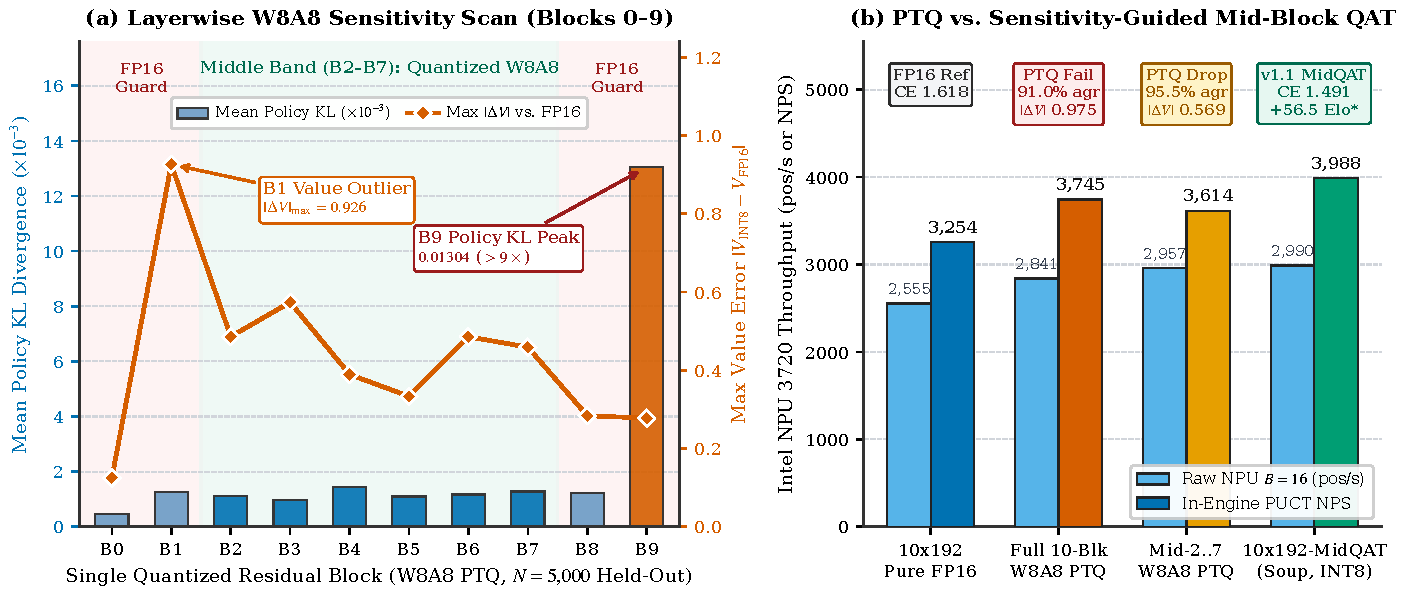
\includegraphics[width=\textwidth]{figures/fig1_block_sensitivity.pdf}
  \caption{\textbf{Sensitivity-Guided Mixed-Precision Quantization on Intel NPU 3720.} (a) Single-block W8A8 PTQ scan across \texttt{block\_0}--\texttt{block\_9} of \texttt{10x192} evaluated on $5{,}000$ \texttt{Far-Test} positions reveals two sharp boundary cliffs: \texttt{block\_9} triggers a $>9\times$ policy KL divergence spike ($0.013042$), while \texttt{block\_1} causes a $0.926$ maximum value error. (b) Throughput and quality comparison across pure FP16, uniform 10-block PTQ, Hybrid Middle-Block (\texttt{2..7}) PTQ, and joint Middle-Block W8A8 QAT (\texttt{A2}), showing how QAT unlocks $3{,}988$\,NPS while simultaneously lowering policy CE ($1.618 \to 1.491$) and gaining $+56.5$\,Elo.}
  \label{fig:block_sensitivity}
\end{figure*}

\subsection{Failure of Uniform W8A8 Quantization}
On Intel NPU~3720, INT8 multiply-accumulate arrays offer nearly double the peak throughput of FP16, making W8A8 quantization an appealing route to deeper real-time search. Yet applying standard uniform post-training quantization (\texttt{nncf.quantize} with fast bias correction~\cite{nagel2020adaround,openvino2024}) across all 10 residual blocks (\texttt{Full\_10Block\_W8A8}) failed catastrophically: on $5{,}000$ held-out \texttt{Far-Test} positions, policy Top-1 agreement against FP16 fell to $90.96\%$, mean policy KL divergence reached $0.021977$, and maximum value error $\max_s |V_{\mathrm{INT8}}(s) - V_{\mathrm{FP16}}(s)|$ hit \textbf{$0.97510$}---nearly a complete $[-1,+1]$ win-to-loss inversion. Weight-only \texttt{W8A16\_ASYM} compression ($6.71$\,MB) degraded agreement to $97.28\%$ while running \emph{slower} than FP16 ($2{,}479.0$ vs.\ $2{,}592.2$ added visits/s) due to runtime dequantization overhead. Even a 20\,M-position uniform 10-block QAT fine-tune reached only $92.52\%$ Top-1 agreement and lost \textbf{$-6.0\%$} in 50-game Stockfish~19 \texttt{UCI\_Elo 3000} matches ($43.0\%$ vs.\ $49.0\%$) despite an $+18.94\%$ NPS boost ($4{,}105$ vs.\ $3{,}452$\,NPS).

\subsection{Layerwise Sensitivity Scan (\texttt{block\_0}--\texttt{block\_9})}
To diagnose the root cause of uniform W8A8 degradation, we performed an isolated single-block quantization scan across all 10 residual blocks of \texttt{Full 346M 10x192} using NNCF \texttt{IgnoredScope} masks calibrated on 500 real positions and measured against FP16 over $5{,}000$ \texttt{Far-Test} positions. For each block $k \in \{0,\dots,9\}$, we recorded Top-1 policy agreement, mean legal-masked policy KL divergence $D_{\mathrm{KL}}(P_{\mathrm{FP16}} \| P_k)$, and maximum absolute value deviation $|\Delta V|_{\max}$.

As plotted in Figure~\ref{fig:block_sensitivity}(a), sensitivity is sharply concentrated at the network boundaries:
\begin{itemize}
  \item \textbf{Final Block Policy Cliff (\texttt{block\_9}):} Quantizing \texttt{block\_9} alone causes policy KL divergence to explode to \textbf{$0.013042$}---more than \textbf{$9\times$ higher} than any other block ($0.000462$--$0.001436$ across \texttt{block\_0}--\texttt{block\_8})---dropping Top-1 agreement from ${\sim}98.0\%$ down to $94.20\%$. Because \texttt{block\_9} feeds directly into the unbounded $4{,}672$-logit \texttt{Conv73} head, small INT8 activation clipping perturbs logit margins between competing tactical candidate moves.
  \item \textbf{Early Block Value Cliff (\texttt{block\_1}):} Quantizing \texttt{block\_1} alone triggers a massive \textbf{$0.92645$} maximum value deviation (compared to $0.125$ at \texttt{block\_0} and $0.278$--$0.574$ across \texttt{block\_2}--\texttt{block\_9}). Early layers mix sparse binary $\{0,1\}$ piece planes with the continuous half-move clock plane; activation quantization noise here amplifies across nine downstream residual blocks into catastrophic value outliers.
\end{itemize}

In addition, isolating the residual skip additions (\texttt{.*\_out\_.*}) revealed that keeping both the four boundary blocks (\texttt{0, 1, 8, 9}), all SE gates, \emph{and} residual skip additions in FP16---quantizing only the $3\times 3$ convolutions inside middle blocks \texttt{2..7} (\texttt{Hybrid\_Middle\_2\_to\_7\_ConvOnly})---improved Top-1 agreement from $94.54\%$ to $95.52\%$, lowered policy KL from $0.007087$ to $0.004891$, cut $|\Delta V|_{\max}$ from $0.62988$ to $0.56921$, and increased raw NPU throughput from $2{,}681.3$ to $2{,}849.6$\,pos/s (and $2{,}956.6$\,pos/s in co-resident benchmarks). Remarkably, against Stockfish ground-truth labels on $5{,}000$ \texttt{Far-Test} positions, \texttt{Hybrid\_Mid2..7} PTQ matched Pure FP16 ($50.54\%$ vs.\ $50.46\%$ Top-1; $0.06085$ vs.\ $0.06117$ value MSE). Yet in actual 50-game Stockfish~19 \texttt{UCI\_Elo 3000} matches, un-retrained \texttt{Hybrid\_Mid2..7} PTQ still collapsed to \textbf{$33.0\%$} (and $25.0\%$ on slice \texttt{[75:85]}) versus $45.0\%$ for Pure FP16, exposing a critical gap between static offline metrics and closed-loop MCTS stability.

\subsection{Joint Middle-Block W8A8 QAT and the $2\times2$ Causal Proof}
To eliminate closed-loop PTQ quantization drift without sacrificing NPU speed, we implemented zero-sync CUDA-native fake-quantization wrappers (\texttt{W8A8FakeQuantConv2d}) exclusively on the $3\times 3$ convolutions of middle blocks \texttt{2..7} (or \texttt{2..9} for \texttt{12x192}) after analytically folding trunk BatchNorms. Each wrapped convolution applies per-output-channel symmetric INT8 weight quantization ($s_w^{(c)} = \max_{i,j,k}|W_{c,i,j,k}| / 127$) and per-tensor exponential moving average (EMA, $\gamma=0.05$) unsigned UINT8 activation quantization ($s_a = a_{\max}^{\mathrm{EMA}}/255$) using the Straight-Through Estimator (STE)~\cite{bengio2013ste,nagel2021whitepaper}:
\begin{align}
  \widehat{W}_c &= s_w^{(c)}\,\mathrm{clip}\!\left(\left\lfloor \frac{W_c}{s_w^{(c)}} \right\rceil,\,-127,\,127\right), \label{eq:wq}\\
  \widehat{X} &= s_a\,\mathrm{clip}\!\left(\left\lfloor \frac{X}{s_a} \right\rceil,\,0,\,255\right), \label{eq:aq}
\end{align}
with backward pass $\partial \widehat{W}/\partial W = I$ and $\partial \widehat{X}/\partial X = I$, while outer blocks (\texttt{0, 1, N-2, N-1}), SE blocks, residual additions, and policy/value/MLH heads remain strictly in FP16/BF16.

\begin{table}[t]
  \centering
  \caption{\textbf{$2\times2$ Causal Factorial vs.\ Stockfish~19 \texttt{UCI\_Elo 3000}} (50g/arm, \texttt{openings\_320[75:100]}, 400\,ms/move, Ponder + Syzygy). Joint Mid-Block W8A8 QAT reverses the PTQ drop into score, NPS, and endgame gains.}
  \label{tab:factorial}
  \resizebox{\columnwidth}{!}{%
  \begin{tabular}{@{}llcccc@{}}
    \toprule
    \textbf{Trunk Regime} & \textbf{Precision} & \textbf{Score} & \textbf{W--D--L} & \textbf{NPS} & \textbf{EG L} \\
    \midrule
    \texttt{346M} Ref (Scalar) & Pure FP16 & 45.0\% & 16--13--21 & 3,292.9 & 7 \\
    \midrule
    Frozen (\texttt{A1} HL64) & Pure FP16 & 33.0\% & 7--19--24 & 3,245.2 & 13 \\
    Frozen (PTQ, no QAT) & Mid-2..7 INT8 & 33.0\%$^\dagger$ & 6--21--23 & 3,980.0 & 11 \\
    \midrule
    Joint (\texttt{A2} HL64) & Pure FP16 & 39.0\% & 9--21--20 & 3,335.3 & 7 \\
    \textbf{Joint (\texttt{A2} HL64)} & \textbf{Mid-2..7 QAT} & \textbf{41.0\%} & \textbf{10--21--19} & \textbf{3,873.9} & \textbf{5} \\
    \bottomrule
    \multicolumn{6}{@{}l@{}}{\scriptsize $^\dagger$Collapsed further to $25.0\%$ ($2\text{W}\text{--}6\text{D}\text{--}12\text{L}$) on diagnostic slice \texttt{[75:85]}.}
  \end{tabular}}
\end{table}

Table~\ref{tab:factorial} and Figure~\ref{fig:qat_sprt}(a) present the controlled $2\times2$ factorial crossing $\{\text{Frozen Trunk vs.\ Joint Trunk}\} \times \{\text{Pure FP16 vs.\ Mid-2..7 INT8}\}$ over 50 paired Stockfish~19 \texttt{UCI\_Elo 3000} games. Under a frozen trunk, Mid-2..7 PTQ degrades playing strength by $-12.0\%$ ($45.0\% \to 33.0\%$, and $-20.0\%$ on slice \texttt{[75:85]}) despite reaching $3{,}980.0$\,NPS. Training the trunk jointly with Middle-Block W8A8 QAT (\texttt{A2}, 40\,M blended positions) completely reverses the sign of quantization: moving from \texttt{A2 FP16} to \texttt{A2 Mid-2..7 QAT INT8} raises match score by \textbf{$+2.0\%$ ($39.0\% \to 41.0\%$)}, increases search throughput by \textbf{$+16.2\%$ ($3{,}335.3 \to 3{,}873.9$\,NPS)}, and cuts late endgame losses from $7$ to $5$. Most decisively, in direct head-to-head NPU matches against the \texttt{346M 10x192} Pure FP16 baseline (Section~\ref{sec:eval}), \texttt{A2 Mid-2..7 QAT INT8} wins by \textbf{$+56.5$\,Elo} ($58.06\%$ over 180 games).

\subsection{Zero-Retraining Weight Souping (\texttt{A2\_soup75})}
Offline zero-search puzzle diagnostics revealed a subtle trade-off after 40\,M joint fine-tuning on the blended Lc0/Stockfish stream: while \texttt{A2} slashed \texttt{far\_test} policy CE from $1.5659$ to $1.4589$ and dramatically improved endgame value calibration, its raw zero-search ($0\text{n}$) tactical puzzle accuracy dipped from $71.5\%$ (\texttt{346M}) to $68.17\%$ because soft Lc0 T80 targets slightly smoothed sharp tactical policy peaks. Following Model Soups~\cite{wortsman2022modelsoups}, we formed a linear weight-space interpolation across all shared stem, residual-block, and \texttt{Conv73} tensors between \texttt{A2} and its \texttt{346M} parent while keeping \texttt{A2}'s \texttt{HL-Gauss-64} and \texttt{MLH} heads intact:
\begin{equation}
  \theta_{\mathrm{soup}}(\alpha) = \alpha\,\theta_{\mathrm{A2}} + (1 - \alpha)\,\theta_{\mathrm{346M}}, \qquad \alpha = 0.75,
  \label{eq:soup}
\end{equation}
followed by clean \texttt{gpu\_unpack} NNCF recalibration (\texttt{A2\_recalib}) on 2,000 real positions. Table~\ref{tab:synthesis} compares all five zero-retraining local synthesis candidates on Intel NPU~3720.

\begin{table}[t]
  \centering
  \caption{\textbf{Zero-Retraining Local Synthesis on Intel NPU 3720} ($5{,}000$ \texttt{test\_far} positions and $1{,}979$ clean Lichess puzzles). \texttt{A2\_soup75} recovers policy sharpness while preserving QAT calibration and ${\sim}3{,}000$\,pos/s speed.}
  \label{tab:synthesis}
  \resizebox{\columnwidth}{!}{%
  \begin{tabular}{@{}lcccc@{}}
    \toprule
    \textbf{Candidate} & \textbf{Far5k CE / MSE} & \textbf{0n Pz} & \textbf{200n Pz} & \textbf{Raw $B{=}16$} \\
    \midrule
    \texttt{A2\_base} (S3) & 1.4879 / 0.05697 & 68.17\% & 82.67\% & 2,890.2 \\
    \texttt{A2\_recalib} & \textbf{1.4874} / \textbf{0.05691} & 68.62\% & 82.77\% & \textbf{3,000.8} \\
    \texttt{A2\_detrunc} ($\times 1.038$) & 1.4874 / 0.05766 & 68.62\% & 82.67\% & 3,000.4 \\
    \textbf{\texttt{A2\_soup75} ($\alpha{=}0.75$)} & 1.4911 / 0.05725 & \textbf{68.72\%} & \textbf{83.07\%} & 2,989.8 \\
    \texttt{A2\_pol\_graft} & 1.4900 / 0.05691 & 68.17\% & 83.02\% & 2,980.2 \\
    \bottomrule
  \end{tabular}}
\end{table}

\texttt{A2\_soup75} achieved the highest clean puzzle solve rate at both $0\text{n}$ ($68.72\%$, $1{,}360/1{,}979$) and $200\text{n}$ ($83.07\%$, $1{,}644/1{,}979$), retained $2{,}989.8$\,pos/s raw $B=16$ throughput ($5.352$\,ms), and defeated \texttt{A2\_base} head-to-head by \textbf{$54.00\%$} ($16\text{W}\text{--}22\text{D}\text{--}12\text{L}$, pentanomial $[0,6,11,6,2]$, \emph{zero} double-losses across 25 opening pairs), earning promotion as the \texttt{v1.1.0} flagship.

% =========================================================================
\section{Distributional Value (\texttt{HL-Gauss-64}) and Decoupled Spot FinOps}
\label{sec:hlgauss}
% =========================================================================

\subsection{Formulation, Expectation Anchoring, and Boundary Truncation}
Post-mortem depth-14 Stockfish audits of 44 losses in \texttt{v1.0.0} revealed that $43.18\%$ ($19/44$) occurred despite Stockfish's best move already lying inside Policy Top-3---indicating that scalar $\tanh$ MSE value regression suffered from zero-shrinkage and weak gradients in sharp tactical positions. Replacing scalar regression with categorical Histogram Loss with Gaussian smoothing (\texttt{HL-Gauss})~\cite{imani2018hlgauss,farebrother2024stop} resolves this pathology at virtually zero NPU compute cost.

We map raw centipawn evaluation $c$ into $v = \tanh(c \cdot \frac{\ln 10}{800}) \in [-1, 1]$ and partition the interval into $K = 64$ bins with uniform centers $z_i = -1 + \frac{2i}{K-1}$ ($i \in \{0,\dots,63\}$), bin width $w = \frac{2}{63} \approx 0.03175$, outer-padded bin edges $e_j = -1 - \frac{w}{2} + jw$ ($j \in \{0,\dots,64\}$), and smoothing width $\sigma = 1.5w \approx 0.04762$. The target categorical distribution $q(v) \in \Delta^{63}$ integrates a truncated Gaussian centered at $v$ over each bin via the standard normal CDF $\Phi$:
\begin{align}
  \tilde{q}_i(v) &= \Phi\!\left(\frac{e_{i+1} - v}{\sigma}\right) - \Phi\!\left(\frac{e_i - v}{\sigma}\right), \nonumber\\
  q_i(v) &= \frac{\tilde{q}_i(v)}{\sum_{m=0}^{63} \tilde{q}_m(v)}.
  \label{eq:hlgauss}
\end{align}
The value head (\texttt{Conv1x1(C,16)} $\to$ \texttt{Linear(1024,256)} $\to$ \texttt{Linear(256,64)}) emits logits $\ell_v \in \mathbb{R}^{64}$ with predicted probabilities $p = \mathrm{softmax}(\ell_v)$ and folded scalar expectation $\hat{v} = \sum_{i=0}^{63} p_i z_i$ computed directly inside the OpenVINO graph. Alongside \texttt{HL-Gauss-64}, an auxiliary Moves-Left Head (\texttt{Conv1x1(C,8)} $\to$ \texttt{Linear(512,64)} $\to$ \texttt{Linear(64,1)} $\to$ \texttt{ReLU}) predicts remaining game plies $\hat{m}(s)$ on shards with game-length labels. The full Phase~4 multi-task objective combines top-8 soft policy cross-entropy, \texttt{HL-Gauss-64} cross-entropy anchored by an explicit expectation MSE regularizer ($\lambda_{\mathrm{mse}} = 2.0$), and masked Smooth-$L_1$ MLH regression:
\begin{align}
  \mathcal{L} &= w_{\mathrm{pol}}\,\mathcal{L}_{\mathrm{pol}}
  + w_{\mathrm{val}}\!\left(\mathcal{L}_{\mathrm{HL\text{-}CE}}(p, q(v)) + 2.0\,(\hat{v} - v)^2\right) \nonumber\\
  &\quad + w_{\mathrm{mlh}}\,\mathcal{L}_{\mathrm{SmoothL1}}\!\left(\frac{\hat{m}}{50},\,\frac{m}{50}\right).
  \label{eq:loss}
\end{align}

\paragraph{Hardware Cost and Boundary Truncation.}
Benchmarking compiled OpenVINO FP16 IRs on Intel NPU~3720 ($B=16$, 200 timed iterations) confirmed that upgrading from scalar $\tanh$ (\texttt{6.386\,ms}, \texttt{13.36\,MB} IR) to \texttt{HL-Gauss-64 + MLH} (\texttt{6.399\,ms}, \texttt{13.44\,MB} IR) incurs just \textbf{$+0.012$\,ms ($+0.19\%$)} latency overhead because the dense value projections fit completely inside L1/CMX cache. On held-out \texttt{test\_far} endgames ($\le 12$ pieces), \texttt{HL-Gauss-64} reduced value MSE from $0.07172$ to $0.06548$ (\texttt{A2}) and $0.05950$ (\texttt{12x192}) while raising endgame decisive sign accuracy from $96.93\%$ to $98.62\%$--$98.84\%$.

An important mathematical property of Eq.~\eqref{eq:hlgauss} is \emph{boundary truncation}: as $v \to +1$, Gaussian mass above $e_{64} = 1 + w/2$ is truncated and renormalized over the left tail, pulling the ideal target expectation inward to $\mathbb{E}_{q(+1)}[z] = 0.9704$ (or $0.9606$ under unpadded $[-1,1]$ edges; empirically saturating near $\pm 0.962$ under noisy targets). We tested post-hoc de-truncation (\texttt{A2\_detrunc}, rescaling support points $z_i \leftarrow 1.038\,z_i$) in Table~\ref{tab:synthesis}; however, \texttt{A2\_detrunc} \emph{regressed} \texttt{test\_far} MSE ($0.05691 \to 0.05766$) and $200\text{n}$ puzzle solve rate ($82.77\% \to 82.67\%$) because the $2.0\,(\hat{v} - v)^2$ expectation-anchoring term in Eq.~\eqref{eq:loss} already compensates for interior bias, causing scalar post-rescaling to overshoot calibrated middlegame evaluations.

\subsection{Three-Tier Decoupled Spot FinOps Pipeline}
To train both \texttt{Job~A} ($40$\,M positions, \texttt{10x192}) and \texttt{Job~B} ($300$\,M positions, \texttt{12x192}) under a strict personal-budget ceiling ($<\$75$), we engineered a decoupled three-tier cloud architecture on AWS SageMaker Managed Spot (\texttt{us-east-1}):
\begin{enumerate}
  \item \textbf{Tier 1 --- High-Throughput C++23 CPU Harvesters:} Rather than burning expensive GPU cycles decompressing \textsc{Lc0} T80 v6 training archives in Python, we wrote a zero-dependency C++23 \texttt{lc0\_v6\_converter} achieving \textbf{$445{,}067$ written pos/s} sustained locally ($0$ illegal moves, max policy probability sum error $1.38 \times 10^{-7}$, max 18-plane error $5.96 \times 10^{-8}$ across 500 parity boards). Deployed across two \texttt{ml.c5.4xlarge} Spot instances ($32$ vCPUs total), the harvesters streamed at $134{,}732$ aggregate pos/s to upload $60 \times 2\text{M}$ blended shards ($70\%$ Lc0 T80 top-8 policy + MLH / $30\%$ Stockfish, $19.74$\,GB total) to S3 for \textbf{${\sim}\$0.14$}.
  \item \textbf{Tier 2 --- Prefetched BF16 Spot GPU Workers:} Training workers on \texttt{ml.g6e.xlarge} (NVIDIA L40S 48\,GB Spot) and \texttt{ml.g5.2xlarge} (A10G 24\,GB Spot) used BF16 AMP, \texttt{channels\_last} memory format, \texttt{torch.compile}, and double-buffered asynchronous S3 shard prefetching, sustaining $63{,}331$\,pos/s for frozen-trunk \texttt{A1}, $9{,}904$\,pos/s for \texttt{A2} fake-quantized QAT, and $33{,}269$\,pos/s ($280$\,M BF16) + $25{,}687$\,pos/s ($20$\,M QAT) for \texttt{Job~B 12x192}.
  \item \textbf{Tier 3 --- Automated IAM FinOps Guardrails:} An independent watchdog (\texttt{NeuraChessGuard}) enforces hard spend limits (auto-attaching an IAM deny-all policy at $\$75$ and terminating jobs at $\$82$). Across all stages of \textsc{NeuraChess} development (including both Phase~4 Spot jobs), conservative cumulative cloud spend totaled \textbf{$\$63.59$} (${\sim}\$16.6$ Phase~4 delta over $\$47.02$ prior spend), with IAM re-frozen immediately upon artifact download.
\end{enumerate}

% =========================================================================
\section{Co-Resident Static-Graph Gear-Shifting vs.\ Pondered Double-Buffering}
\label{sec:gearshift}
% =========================================================================

\subsection{Sub-Linear NPU Latency and Co-Resident Footprint}
Static profiling of Intel NPU~3720 across batch sizes reveals a strongly sub-linear turnaround latency curve: for \texttt{10x192} Pure FP16 (\texttt{Hybrid Mid-2..7 INT8}), median latencies are $0.739$\,ms ($0.708$\,ms) at $B=1$, $1.894$\,ms ($1.603$\,ms) at $B=4$, $3.360$\,ms ($2.859$\,ms) at $B=8$, and $6.262$\,ms ($5.412$\,ms) at $B=16$. Consequently, $B=4$ executes \textbf{$3.38\times$ faster} per sequential wave than $B=16$ while preserving \textbf{$84.4\%$} of raw throughput ($2{,}495.6$ vs.\ $2{,}956.6$\,pos/s), and $B=8$ runs $1.89\times$ faster at $94.6\%$ of peak throughput ($2{,}797.8$\,pos/s).

Crucially, OpenVINO permits compiling all four static graphs ($B\in\{1,4,8,16\}$) simultaneously \emph{co-resident} on the NPU with minimal memory overhead: total NPU device allocation grows monotonically from $13.70$\,MB ($B=1$) to $27.95$\,MB ($+B=4$), $42.88$\,MB ($+B=8$), and just \textbf{$59.09$\,MB} across all four graphs ($172.38$\,MB host RSS delta out of $8{,}192$\,MB addressable device memory).

\subsection{Collision-Bounded \texttt{gear\_shift\_v3} and Cold-Start Gains}
Naive entropy-gated batch switching over-triggered $B=4$ on $94.4\%$ of batches in open middlegames, sacrificing node volume. Refining the C++23 scheduler into \texttt{gear\_shift\_v3} replaced heuristic entropy triggers with three structural rules: (i) \emph{Cold-Start Ramp} ($N_{\mathrm{root}} < 16 \Rightarrow B=4$), (ii) \emph{Capped Narrow Root} (in check or $\le 5$ legal moves with $N_{\mathrm{root}} < 32 \Rightarrow B=4$), and (iii) \emph{Collision-Bounded Flush} (during \texttt{select(16)}, once $\ge 6$ virtual-loss collisions or cache/terminal hits occur, immediately dispatch $B=4$ for $1\text{--}4$ unique uncached leaves or $B=8$ for $5\text{--}8$ leaves rather than padding to $16$).

In cold-start tactical regimes (empty tree at turn start), \texttt{gear\_shift\_v3} produces striking gains (Figure~\ref{fig:puzzles_ladder}(b)):
\begin{itemize}
  \item \textbf{Mate-in-3 ($n=100$, $400$\,ms):} Maintains $97/100$ solve rate while cutting total wall time from $7.25$\,s to \textbf{$2.30$\,s ($3.15\times$ speedup)}, reducing mean evaluated nodes per puzzle from $190.28$ to $43.13$ and increasing average search ply from $1.739$ to $2.192$.
  \item \textbf{Ultra-Fast Clean Puzzles ($n=500$):} At $50$\,ms/move, combining \texttt{gear\_shift\_v3} with \texttt{Hybrid Mid-2..7 INT8} boosts solve rate by \textbf{$+8.0\%$ ($80.0\% \to 88.0\%$)}, lifting average search depth from $2.21$ to $3.35$\,plies (max ply $4.33 \to 7.12$). At $100$\,ms/move, accuracy jumps \textbf{$+7.0\%$ ($85.6\% \to 92.6\%$)}, with $2100+$ master puzzles rising from $69\%$ to $80\%$ ($+11\%$).
\end{itemize}

\subsection{Why Static $B=16$ Double-Buffering Wins Under Pondering}
Despite its dramatic cold-start puzzle advantage, controlled match ablations revealed an important regime boundary: under $400$\,ms/move games with \emph{pondering enabled}, enabling \texttt{gear\_shift\_v3} degraded Pure FP16 score against Stockfish~19 \texttt{UCI\_Elo 3000} from $45.0\%$ to $30.0\%$ ($3\text{W}\text{--}6\text{D}\text{--}11\text{L}$ on slice \texttt{[75:85]}). Telemetry pinpointed two interacting mechanisms: first, opponent-turn pondering already pre-populates an average of $785.7$ retained root visits (far above the $N_{\mathrm{root}} < 32$ ramp threshold), so $>80\%$ of batches already execute at $B=16$; second, transitioning between distinct compiled graphs stalls the \texttt{nireq=2} asynchronous double-buffering pipeline that overlaps CPU selection behind NPU inference. Production search therefore automatically gates dynamic gear-shifting via \texttt{allow\_gear\_shift = (not use\_ponder) or (movetime\_ms <= 150)}, capturing cold-start/bullet tactical gains while preserving peak double-buffered throughput during pondered play.

% =========================================================================
\section{Compute-Optimal NPU Scaling and Rigorous Negative Results}
\label{sec:scaling}
% =========================================================================

\begin{figure*}[t]
  \centering
  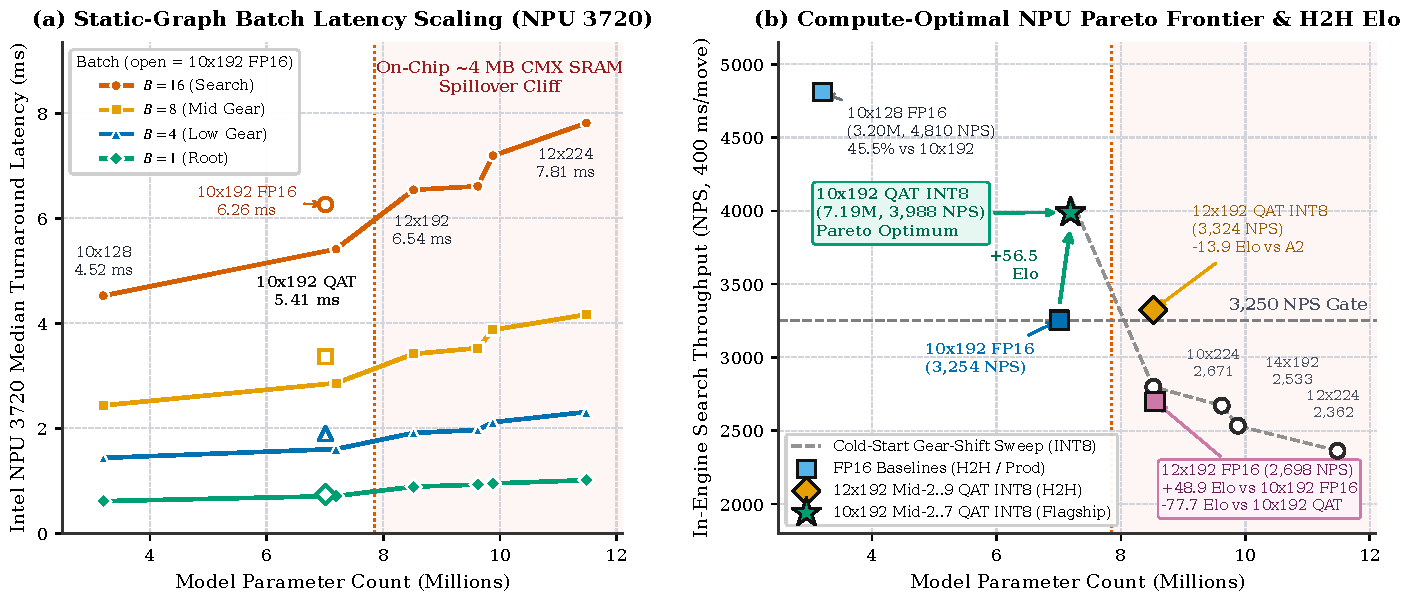
\includegraphics[width=\textwidth]{figures/fig2_npu_pareto_frontier.pdf}
  \caption{\textbf{Intel NPU 3720 Scaling Curves and the CMX SRAM Pareto Cliff.} (a) Median turnaround latency across $B\in\{1,4,8,16\}$ from \texttt{10x128} ($3.20$\,M) to \texttt{12x224} ($11.48$\,M); crossing ${\sim}7.85$\,M parameters triggers a steep latency jump as weights and activations spill beyond the ${\sim}4$\,MB on-chip CMX SRAM. (b) Real-time in-engine NPS ($400$\,ms/move) vs.\ parameter count overlaid with paired head-to-head Elo outcomes. Although \texttt{12x192 FP16} defeats \texttt{10x192 FP16} by $+48.9$\,Elo, it loses by $-77.7$\,Elo to \texttt{10x192 QAT INT8} ($3{,}988$\,NPS), and even \texttt{12x192 QAT INT8} ($3{,}324$\,NPS) trails by $-13.9$\,Elo, placing \texttt{10x192 QAT INT8} at the hardware Pareto optimum.}
  \label{fig:npu_pareto}
\end{figure*}

\subsection{Function-Preserving Depth Expansion (\texttt{10x192}\,$\to$\,\texttt{12x192})}
To test whether increasing neural capacity could surpass \texttt{10x192} under fixed $400$\,ms NPU time controls, we swept four candidate architectures (\texttt{12x192}, \texttt{10x224}, \texttt{14x192}, \texttt{12x224}) on NPU~3720 with middle-block W8A8 quantization and \texttt{HL-Gauss-64}. All four failed the $3{,}250$\,NPS cold-start gate (Figure~\ref{fig:npu_pareto}), with \texttt{12x192\_mid2\_9\_hl64} ($8.52$\,M backbone params, $8.55$\,M with MLH, $B=16$ latency $6.540$\,ms) coming closest.

Rather than training \texttt{12x192} from scratch, we initialized \texttt{Job~B} via function-preserving \texttt{Net2DeeperNet}~\cite{chen2016net2net} residual block injection from the converged \texttt{346M 10x192} checkpoint: stem, \texttt{Conv73} policy, and blocks $0\text{--}9$ were copied into indices $\{0,1,2,3,4,6,7,8,9,10\}$, while new blocks at indices $5$ and $11$ initialized \texttt{conv1} via Kaiming normal and set \texttt{conv2} weights/biases to zero with identity \texttt{bn2}, guaranteeing $x + \mathrm{SE}(0) = x$. Verification prior to Step~0 confirmed exact \textbf{$0.000\text{e}{+}00$} maximum policy logit drift across evaluation splits.

\subsection{The CMX SRAM Latency Cliff and Elo Inversion}
After $280$\,M BF16 positions plus $20$\,M Stage-3 Middle-Block (\texttt{2..9}) W8A8 QAT, \texttt{12x192} achieved our strongest offline metrics across every split: $1.4428$ (\texttt{ema\_09995}) and $1.4474$ (\texttt{qat\_mid2\_9}) \texttt{far\_test} policy CE, and best-in-class OOD endgame value MSE ($0.05684$, $98.84\%$ decisive sign accuracy). Table~\ref{tab:scaling} summarizes the complete architectural frontier.

\begin{table}[t]
  \centering
  \caption{\textbf{Intel NPU 3720 Architecture Scaling Sweep.} Latencies are median turnaround (ms) under \texttt{LATENCY} + \texttt{NPU\_TURBO}. Beyond ${\sim}8$\,M parameters, CMX SRAM spillover compresses search NPS below the \texttt{10x192 QAT INT8} Pareto knee.}
  \label{tab:scaling}
  \resizebox{\columnwidth}{!}{%
  \begin{tabular}{@{}lcccccc@{}}
    \toprule
    \textbf{Architecture} & \textbf{Params} & \textbf{$B{=}1$} & \textbf{$B{=}4$} & \textbf{$B{=}8$} & \textbf{$B{=}16$} & \textbf{Eng.\ NPS} \\
    \midrule
    \texttt{10x128} FP16 & 3.20\,M & 0.611 & 1.434 & 2.434 & 4.523 & 4,810.4 \\
    \texttt{10x192} FP16 & 7.01\,M & 0.739 & 1.894 & 3.360 & 6.262 & 3,253.9 \\
    \textbf{\texttt{10x192} QAT INT8} & \textbf{7.19\,M} & \textbf{0.708} & \textbf{1.603} & \textbf{2.859} & \textbf{5.412} & \textbf{3,987.9} \\
    \texttt{12x192} QAT INT8 & 8.52\,M & 0.886 & 1.910 & 3.415 & 6.540 & 3,324.0$^\star$ \\
    \texttt{10x224} INT8 & 9.62\,M & 0.925 & 1.966 & 3.526 & 6.609 & 2,670.5$^\dagger$ \\
    \texttt{14x192} INT8 & 9.88\,M & 0.948 & 2.114 & 3.872 & 7.189 & 2,533.0$^\dagger$ \\
    \texttt{12x224} INT8 & 11.48\,M & 1.010 & 2.308 & 4.164 & 7.813 & 2,362.3$^\dagger$ \\
    \bottomrule
    \multicolumn{7}{@{}l@{}}{\scriptsize $^\star$H2H $B{=}16$ NPS ($2{,}798.7$ cold gear-shift). $^\dagger$Cold-start gear-shift sweep NPS.}
  \end{tabular}}
\end{table}

Paired $400$\,ms/move head-to-head NPU matches exposed a dramatic hardware-induced Elo inversion (Figure~\ref{fig:npu_pareto}(b)):
\begin{itemize}
  \item \textbf{FP16 vs.\ FP16:} \texttt{12x192 ema\_09995 FP16} defeated \texttt{346M 10x192 FP16} by \textbf{$+48.9$\,Elo ($57.0\%$, $22\text{W}\text{--}13\text{D}\text{--}15\text{L}$)} despite running $16.9\%$ slower ($2{,}698.4$ vs.\ $3{,}246.0$\,NPS)---showing that deeper value/policy capacity outweighs a modest FP16 speed deficit.
  \item \textbf{Against \texttt{10x192 QAT INT8}:} When facing \texttt{A2 10x192 QAT INT8} ($3{,}803.4$\,NPS), \texttt{12x192 FP16} collapsed to \textbf{$39.0\%$ ($-77.7$\,Elo, $11\text{W}\text{--}17\text{D}\text{--}22\text{L}$)}. Even after applying Middle-Block (\texttt{2..9}) W8A8 QAT to \texttt{12x192} (boosting its NPS by $+24.3\%$ to $3{,}324.0$\,NPS and recovering $+64$\,Elo), \texttt{12x192 QAT INT8} still trailed \texttt{A2 10x192 QAT INT8} at \textbf{$48.0\%$ ($-13.9$\,Elo, $16\text{W}\text{--}16\text{D}\text{--}18\text{L}$)}.
\end{itemize}
On the smaller side, \texttt{10x128 FP16} ($3.20$\,M, $4{,}810.4$\,NPS) scored only $45.5\%$ against \texttt{10x192 FP16} ($3{,}290.3$\,NPS) in 100 paired games because its reduced channel capacity increased policy CE by $+0.0541$ across 150k benchmark positions. Thus, \texttt{10x192 Mid-2..7 QAT INT8} sits precisely at the compute-optimal Pareto knee of Intel NPU~3720, maximizing the product of representation quality and on-chip SRAM search throughput.

\subsection{Rigorous Negative Results}
Documenting principled failures is essential for reproducible edge-AI engineering. Alongside uniform PTQ/W8A16 and \texttt{A2\_detrunc}, three additional negative results shaped our final architecture:

\paragraph{1. 37.85\,ns Bitboard SEE Prior Shaping (``The Bitter Lesson'').}
To exploit the $91.44\%$ CPU idle window without staleness, we implemented an exact C++23 Static Exchange Evaluator (\texttt{CBoard::see()}) handling X-ray slider discovery, pinned defenders, en passant, and promotion recaptures. It passed $56/56$ tactical unit tests at \textbf{$37.85$\,ns/call} ($0.0378\,\mu$s) and was wired into an AVX2 \texttt{fpu\_bias} lane applying a $-0.15$ FPU penalty to losing low-prior captures ($\mathrm{SEE} < -100$\,cp, $P < 0.15$) and $+0.05$ FPU boost to winning captures ($\mathrm{SEE} \ge +100$\,cp). Across every benchmark, SEE shaping \emph{degraded} accuracy: on 500 stratified Lichess puzzles, accuracy dropped from $78.80\%$ to $78.20\%$ at $50\text{n}$ ($394 \to 391$) and from $82.20\%$ to $82.00\%$ at $200\text{n}$ ($411 \to 410$); on 19 tactical-horizon losses (\texttt{Cat~C}, $200\text{n}$), mean centipawn drop worsened from $127.16$ to $134.42$\,cp ($\ge 150$\,cp blunders $6 \to 7$); on 19 value-search losses (\texttt{Cat~A}, $200\text{n}$), mean drop worsened from $33.63$ to $38.79$\,cp. Echoing Sutton's \emph{Bitter Lesson}~\cite{sutton2019bitter}, static 1-square material accounting systematically penalizes positional sacrifices and overloaded-defender tactics already internalized by the 346\,M-trained policy network. The flag remains permanently disabled (\texttt{use\_see\_prior\_shaping=False}).

\paragraph{2. \texttt{10x128} 50-Node Async Double-Buffering Dispersion.}
Early benchmarks of \texttt{10x128} exhibited an anomalous $-19$-point drop on 50-node puzzles ($58.16\%$) relative to \texttt{6x128} ($70.54\%$) and \texttt{10x192} ($79.38\%$). Controlled single-parameter ablations across all $1{,}979$ clean puzzles ($50\text{n}$, $B=16$) isolated the sole cause to asynchronous double-buffering (\texttt{use\_async\_overlap=True, async\_inflight=2}):
\begin{itemize}
  \item Sequential (\texttt{nireq=1}, $\delta_{\mathrm{fpu}}=0.20$): \textbf{$77.36\%$} ($1{,}531/1{,}979$, $74.87$ avg nodes across $4.40$ sequential waves).
  \item Sequential control ($\delta_{\mathrm{fpu}}=0.25$): \textbf{$77.36\%$} ($1{,}531/1{,}979$) --- zero regression from FPU.
  \item Single-parameter flip to \texttt{nireq=2} ($\delta_{\mathrm{fpu}}=0.20$): \textbf{$58.67\%$} ($1{,}161/1{,}979$, $61.57$ avg nodes across $3.57$ waves) --- an \textbf{$-18.69\%$} collapse ($58.16\%$ with $\delta_{\mathrm{fpu}}=0.25$).
\end{itemize}
Keeping $32$ concurrent virtual-loss leaves in flight under a 50-node budget forces excessive breadth dispersion before deep forcing replies are backed up. Consequently, fixed-node search and non-pondered controls default strictly to sequential execution (\texttt{nireq=1}).

\paragraph{3. Opening Root Top-$K$ Guard and Large Batches.}
Restricting opening root expansion to Policy Top-4 with $P \ge 0.08$ recovered only $22/28$ opening blunders (failing our pre-registered $24/28$ threshold) and was rejected. Likewise, increasing NPU batch size to $B=32$ or $B=64$ degraded equal-time strength to $26.56\%$ and $0.00\%$ against $B=16$, confirming $B=16$ as the upper sequential-staleness limit on edge NPUs.

% =========================================================================
\section{End-to-End Evaluation and Conclusion}
\label{sec:eval}
% =========================================================================

\begin{figure*}[t]
  \centering
  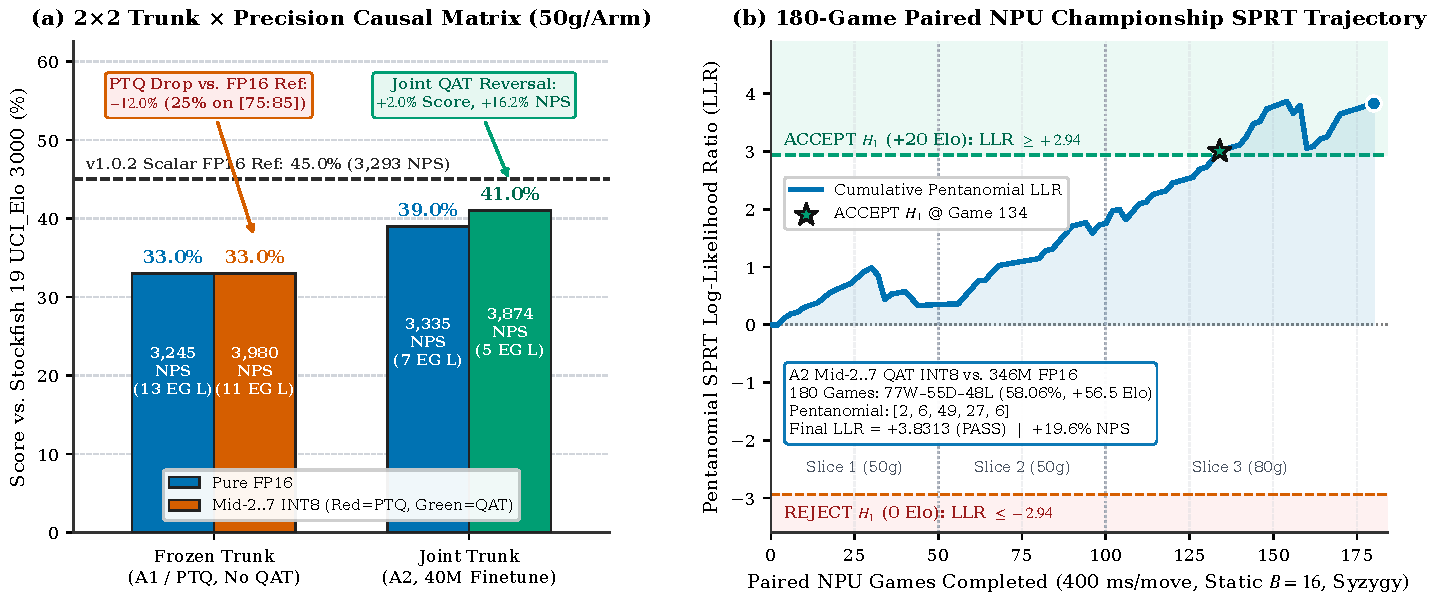
\includegraphics[width=\textwidth]{figures/fig3_qat_factorial_and_sprt.pdf}
  \caption{\textbf{Causal Factorial Proof and 180-Game Pentanomial SPRT Championship.} (a) $2\times2$ factorial vs.\ Stockfish~19 \texttt{UCI\_Elo 3000} ($50$g/arm) isolating why frozen-trunk PTQ collapses ($33.0\%$ vs.\ $45.0\%$ FP16 ref) whereas joint Middle-Block QAT reverses quantization into $+2.0\%$ score, $+16.2\%$ NPS, and fewer endgame losses ($5$ vs.\ $7$). (b) Cumulative pentanomial SPRT log-likelihood ratio across 180 paired NPU games (\texttt{A2 Mid-2..7 QAT INT8} vs.\ \texttt{346M 10x192 FP16}), crossing \texttt{ACCEPT\_H1} ($+20$\,Elo) at Game~134 and finishing at $\mathrm{LLR} = +3.8313$ ($+56.5$\,Elo, $+19.6\%$ NPS).}
  \label{fig:qat_sprt}
\end{figure*}

\begin{figure*}[t]
  \centering
  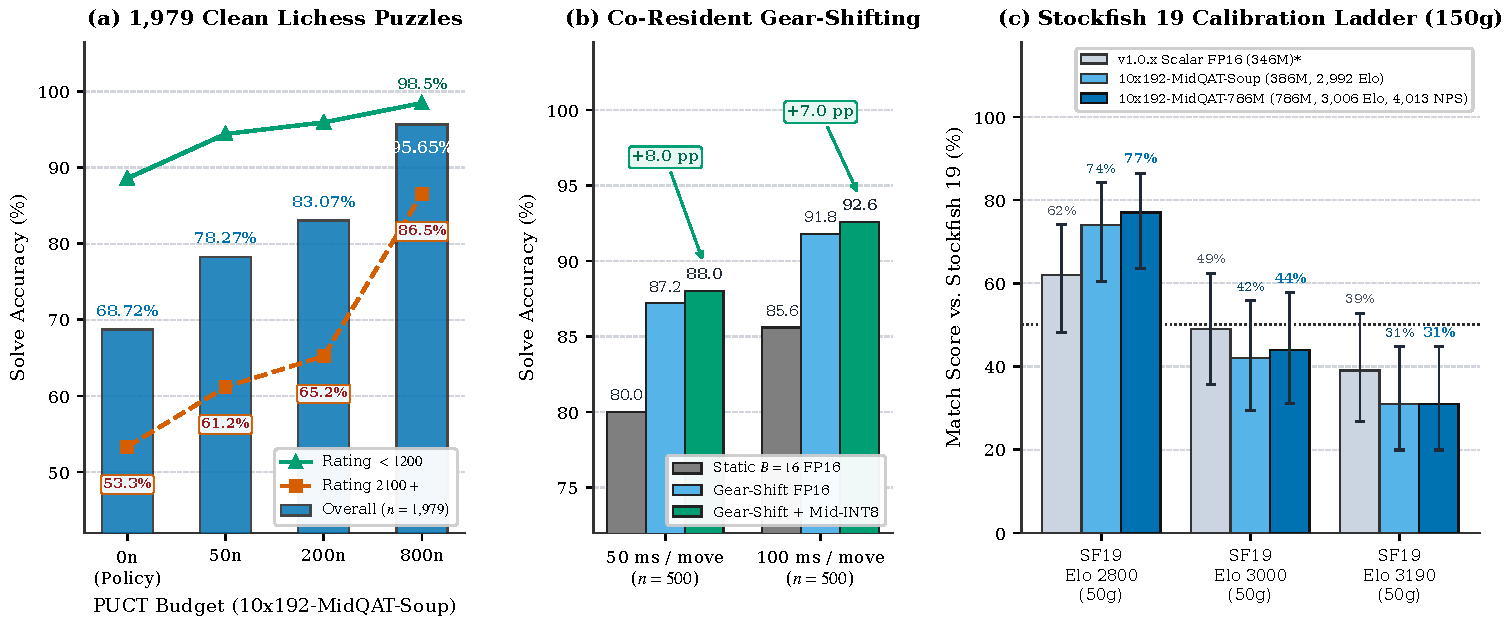
\includegraphics[width=\textwidth]{figures/fig4_puzzles_and_ladder.pdf}
  \caption{\textbf{Tactical Puzzles, Co-Resident Gear-Shifting, and Stockfish~19 Benchmarks.} (a) Clean $1{,}979$ Lichess puzzle scaling for \texttt{v1.1.0} (\texttt{A2\_soup75} INT8) from $68.72\%$ ($0\text{n}$) to $95.65\%$ ($800\text{n}$), including the $2100+$ master bucket ($53.3\% \to 86.55\%$). (b) Co-resident $B\in\{4,8,16\}$ gear-shifting gains on 500 clean puzzles at $50$\,ms ($+8.0\%$) and $100$\,ms ($+7.0\%$). (c) Stockfish~19 calibration ladder ($150$g, mean implied \texttt{UCI\_Elo} $2{,}992$) and uncapped \texttt{go nodes 3500} crossover jump ($37.50\% \to 83.75\%$, $+46.25\%$). $^\ast$\texttt{v1.0.x} ladder used \texttt{OPENINGS\_50}; \texttt{v1.1.0} used disjoint unseen \texttt{openings\_320} slices.}
  \label{fig:puzzles_ladder}
\end{figure*}

\subsection{Statistical Methodology: Pentanomial SPRT}
To eliminate opening-color bias and reduce variance in paired head-to-head NPU matches, each opening position is played twice with reversed colors, yielding a pair score $s_k \in \{0, 0.25, 0.50, 0.75, 1.0\}$ (mapping pair points $\{0, 0.5, 1.0, 1.5, 2.0\}$) aggregated into pentanomial counts $\mathbf{c} = (c_0, c_1, c_2, c_3, c_4)$ over $M = \sum_j c_j$ pairs. Following Fishtest's generalized pentanomial Sequential Probability Ratio Test (SPRT)~\cite{wald1945sprt,stockfish2025}, we compute Jeffreys-smoothed empirical probabilities $\hat{p}_j = (c_j + 0.5)/(M + 2.5)$ and solve via Newton iteration for the exponentially tilted maximum-likelihood distributions $q^{(0)}_j \propto \hat{p}_j e^{\beta_0 x_j}$ and $q^{(1)}_j \propto \hat{p}_j e^{\beta_1 x_j}$ whose means match the logistic Elo hypotheses $\mu(q^{(r)}) = (1 + 10^{-\mathrm{Elo}_r/400})^{-1}$ for $\mathrm{Elo}_0 = 0$ and $\mathrm{Elo}_1 = +20$:
\begin{equation}
  \mathrm{LLR}(\mathbf{c}) = \sum_{j=0}^{4} c_j \ln\!\frac{q^{(1)}_j}{q^{(0)}_j},
  \label{eq:sprt}
\end{equation}
with $\alpha = \beta = 0.05$ stopping bounds $\pm \ln\!\left(\frac{1-\beta}{\alpha}\right) = \pm 2.9444$.

\subsection{180-Game Paired NPU Championship SPRT}
Table~\ref{tab:sprt180} reports the complete 180-game paired head-to-head validation ($90$ disjoint opening pairs \texttt{openings\_320[75:165]}, $400$\,ms/move, static $B=16$, 5-piece Syzygy) comparing \texttt{A2 Mid-2..7 W8A8 QAT INT8} against the \texttt{v1.0.2 346M 10x192} Pure FP16 baseline. Across all three independent slices, \texttt{A2} won consistently ($54.0\%$, $59.0\%$, $60.0\%$), crossing \texttt{ACCEPT\_H1} at pair~67 (Game~134, $\mathrm{LLR}=+3.0048$) and concluding at \textbf{$58.06\%$ ($77\text{W}\text{--}55\text{D}\text{--}48\text{L}$, $+56.5$\,Elo, 95\% Wilson CI $[50.75\%, 65.02\%]$, $\mathrm{LLR} = +3.8313$)} while sustaining $+19.6\%$ higher real-time search throughput ($3{,}890.7$ vs.\ $3{,}253.9$\,NPS).

\begin{table*}[t]
  \centering
  \caption{\textbf{180-Game Paired NPU Championship SPRT} (\texttt{A2 Mid-2..7 QAT INT8} vs.\ \texttt{346M 10x192 FP16}, $400$\,ms/move, static $B=16$, 5-piece Syzygy) and secondary head-to-head NPU verifications.}
  \label{tab:sprt180}
  \resizebox{\textwidth}{!}{%
  \begin{tabular}{@{}lccccccc@{}}
    \toprule
    \textbf{Matchup / Opening Slice} & \textbf{Games} & \textbf{Score (\%)} & \textbf{W--D--L} & \textbf{Elo Diff} & \textbf{Pentanomial} & \textbf{SPRT LLR} & \textbf{NPS (A / B)} \\
    \midrule
    \texttt{A2} vs.\ \texttt{346M} \texttt{[75:100]} & 50 & 54.00 & 17--20--13 & $+27.9$ & $[1, 3, 13, 7, 1]$ & $+0.3501$ & 3,850.0 / 3,239.6 \\
    \texttt{A2} vs.\ \texttt{346M} \texttt{[100:125]} & 50 & 59.00 & 22--15--13 & $+63.2$ & $[0, 1, 14, 10, 0]$ & $+1.7532^\star$ & 3,866.3 / 3,223.2 \\
    \texttt{A2} vs.\ \texttt{346M} \texttt{[125:165]} & 80 & 60.00 & 38--20--22 & $+70.3$ & $[1, 2, 22, 10, 5]$ & $+3.8313^\star$ & 3,931.3 / 3,282.0 \\
    \midrule
    \textbf{Combined SPRT Pass (\texttt{[75:165]})} & \textbf{180} & \textbf{58.06} & \textbf{77--55--48} & \textbf{$+56.5$} & $\mathbf{[2, 6, 49, 27, 6]}$ & \textbf{$+3.8313$ (PASS)} & \textbf{3,890.7 / 3,253.9} \\
    \midrule
    \texttt{A2\_soup75} vs.\ \texttt{A2\_base} \texttt{[75:100]} & 50 & 54.00 & 16--22--12 & $+27.9$ & $[0, 6, 11, 6, 2]$ & $+0.3411$ & 3,583.3 / 3,597.5 \\
    \texttt{12x192 FP16} vs.\ \texttt{346M} \texttt{[75:100]} & 50 & 57.00 & 22--13--15 & $+48.9$ & $[1, 4, 12, 3, 5]$ & $+0.5301$ & 2,698.4 / 3,246.0 \\
    \texttt{12x192 FP16} vs.\ \texttt{A2} \texttt{[75:100]} & 50 & 39.00 & 11--17--22 & $-77.7$ & $[2, 9, 12, 2, 0]$ & $-1.8170$ & 2,673.1 / 3,803.4 \\
    \texttt{12x192 INT8} vs.\ \texttt{A2} \texttt{[75:100]} & 50 & 48.00 & 16--16--18 & $-13.9$ & $[0, 6, 16, 2, 1]$ & $-0.5799$ & 3,324.0 / 3,868.4 \\
    \bottomrule
    \multicolumn{8}{@{}l@{}}{\scriptsize $^\star$Cumulative LLR across slices through Game~100 and Game~180. Combined 95\% Wilson CI: $[50.75\%, 65.02\%]$; SPRT bounds $\pm 2.9444$ ($\mathrm{Elo}_0{=}0, \mathrm{Elo}_1{=}20$).}
  \end{tabular}}
\end{table*}

\subsection{Stockfish 19 Ladder, Fixed-Node Crossover, and Clean Lichess Puzzles}
Table~\ref{tab:sf_ladder} summarizes the official external evaluation of the promoted \texttt{v1.1.0} flagship (\texttt{A2\_soup75} Mid-2..7 QAT INT8) against Stockfish~19 (400\,ms/move, Ponder ON, Syzygy ON, \texttt{OwnBook=False}) across $150$ unseen \texttt{openings\_320[0:75]} ladder games and $40$ uncapped fixed-node crossover games (\texttt{go nodes 3500}, \texttt{openings\_320[165:185]}). Across the three \texttt{UCI\_Elo} tiers ($2800$, $3000$, $3190$), \textsc{NeuraChess} scored $74.00\%$ ($29\text{W}\text{--}16\text{D}\text{--}5\text{L}$, implied $2{,}981.7$), $42.00\%$ ($6\text{W}\text{--}30\text{D}\text{--}14\text{L}$, implied $2{,}943.9$), and $31.00\%$ ($3\text{W}\text{--}25\text{D}\text{--}22\text{L}$, implied $3{,}051.0$), yielding a combined $49.00\%$ ($38\text{W}\text{--}71\text{D}\text{--}41\text{L}$), \textbf{$3{,}987.9$ mean effective NPS}, and \textbf{$2{,}992.2$ mean implied \texttt{UCI\_Elo}}. Most notably, against uncapped Stockfish~19 restricted to \texttt{go nodes 3500} (removing artificial \texttt{UCI\_Elo} weakening noise), \texttt{v1.1.0} surged from \texttt{v1.0.2}'s $37.50\%$ ($9\text{W}\text{--}12\text{D}\text{--}19\text{L}$) to \textbf{$83.75\%$ ($30\text{W}\text{--}7\text{D}\text{--}3\text{L}$, $+46.25\%$ jump)}.

\begin{table*}[t]
  \centering
  \caption{\textbf{Stockfish~19 Calibration Ladder (150g) and Uncapped \texttt{go nodes 3500} Crossover (40g)} for \texttt{v1.1.0} (\texttt{A2\_soup75} INT8, 400\,ms/move, Ponder + Syzygy, unseen \texttt{openings\_320} slices).}
  \label{tab:sf_ladder}
  \footnotesize
  \setlength{\tabcolsep}{5.0pt}
  \begin{tabular}{@{}lcccccc@{}}
    \toprule
    \textbf{Stockfish 19 Tier / Engine} & \textbf{Games} & \textbf{Score (\%)} & \textbf{W--D--L} & \textbf{95\% Wilson CI (\%)} & \textbf{Eff.\ NPS} & \textbf{Implied \texttt{UCI\_Elo}} \\
    \midrule
    \texttt{UCI\_Elo 2800} (\texttt{openings\_320[0:25]}) & 50 & 74.00 & 29--16--5 & $[60.45,\; 84.13]$ & 3,898.9 & 2,981.7 \\
    \texttt{UCI\_Elo 3000} (\texttt{openings\_320[25:50]}) & 50 & 42.00 & 6--30--14 & $[29.37,\; 55.77]$ & 4,025.1 & 2,943.9 \\
    \texttt{UCI\_Elo 3190} (\texttt{openings\_320[50:75]}) & 50 & 31.00 & 3--25--22 & $[19.93,\; 44.78]$ & 4,039.6 & 3,051.0 \\
    \midrule
    \textbf{Combined Ladder (\texttt{v1.1.0} \texttt{A2\_soup75})} & \textbf{150} & \textbf{49.00} & \textbf{38--71--41} & $[41.13,\; 56.92]$ & \textbf{3,987.9} & \textbf{2,992.2} \\
    \midrule
    \texttt{go nodes 3500} (\texttt{v1.0.2} 346M FP16) & 40 & 37.50 & 9--12--19 & $[24.22,\; 52.97]$ & 3,264.6 & --- \\
    \textbf{\texttt{go nodes 3500} (\texttt{v1.1.0} \texttt{A2\_soup75})} & \textbf{40} & \textbf{83.75} & \textbf{30--7--3} & $\mathbf{[69.48,\; 92.11]}$ & \textbf{3,771.0} & --- \\
    \bottomrule
  \end{tabular}
\end{table*}

Finally, Table~\ref{tab:puzzles} details tactical scaling across all $1{,}979$ leakage-free Lichess puzzles (21 training-set overlaps strictly excluded prior to evaluation, Syzygy disabled). Scaling PUCT search from raw policy ($0\text{n}$) to $800\text{n}$ raises overall solve accuracy from $68.72\%$ to \textbf{$95.65\%$ ($1{,}893/1{,}979$)}, lifting the hardest $2100+$ master tier by $+33.25$ percentage points ($53.30\% \to 86.55\%$).

\begin{table*}[t]
  \centering
  \caption{\textbf{Clean Lichess Tactical Puzzle Scaling ($n=1{,}979$, \texttt{v1.1.0} \texttt{A2\_soup75} INT8, Syzygy OFF).} Solve accuracy (\%) across stratified rating buckets and PUCT node budgets.}
  \label{tab:puzzles}
  \small
  \begin{tabular}{@{}lccccccc@{}}
    \toprule
    \textbf{Search Budget} & \textbf{Solved / 1,979} & \textbf{Overall (\%)} & \textbf{$<1200$} & \textbf{1200--1499} & \textbf{1500--1799} & \textbf{1800--2099} & \textbf{$2100+$} \\
    \midrule
    $0\text{n}$ (Raw Policy Top-1) & 1,360 & 68.72 & 88.58 & 72.91 & 67.84 & 61.06 & 53.30 \\
    $50\text{n}$ ($3{,}064.2$\,NPS) & 1,549 & 78.27 & 94.42 & 85.06 & 78.14 & 72.61 & 61.17 \\
    $200\text{n}$ ($3{,}133.5$\,NPS) & 1,644 & 83.07 & 95.94 & 89.62 & 84.17 & 80.40 & 65.23 \\
    \textbf{$800\text{n}$ ($3{,}387.1$\,NPS)} & \textbf{1,893} & \textbf{95.65} & \textbf{98.48} & \textbf{99.24} & \textbf{96.23} & \textbf{97.74} & \textbf{86.55} \\
    \bottomrule
  \end{tabular}
\end{table*}

\subsection{Conclusion and Future Directions}
We have demonstrated that near-3,000-Elo neural MCTS is practical on a 3\,W consumer edge NPU when neural precision, distributional loss geometry, multi-shape compilation, and real-time search control are explicitly co-designed around on-chip SRAM and sequential tree dynamics. Protecting quantization-sensitive boundary blocks (\texttt{0, 1, 8, 9}) and skip connections while training middle blocks (\texttt{2..7}) jointly under W8A8 QAT unlocks $+19.6\%$ throughput and $+56.5$\,Elo over FP16; adding \texttt{HL-Gauss-64 + MLH} costs just $+0.19\%$ NPU latency; and coupling co-resident gear-shifting with clock-aware 4-gear allocation and MCTS early stopping delivers crisp, flag-free bullet play. Promising future avenues include distilling a parallel single-pass \texttt{Conv73} action-value head $Q_\theta(s,a)$ for learned First-Play Urgency (already benchmarked at just $+0.087$\,ms / $+1.36\%$ NPU overhead) and extending MLH-conditioned draw contempt into dynamic time-pressure search control.

{\sloppy
\bibliographystyle{plain}
\bibliography{references}
}

\end{document}
